\documentclass[12pt]{article}

\usepackage{amsmath}
\usepackage{amssymb}
\usepackage{amsthm}
\usepackage{centernot}
\usepackage{fullpage}
\usepackage{makecell}
\usepackage{tabularx}
\usepackage[hypcap=false]{caption}
\usepackage[dvipsnames]{xcolor}
\usepackage{tikz,tkz-euclide}
\usetikzlibrary{decorations.pathreplacing,arrows}
\usetikzlibrary{quotes,angles,calc,intersections}
\usepackage{pgfplots}
\pgfplotsset{compat=1.17}

\usepackage{titling}
\usepackage{pdfpages}
\usepackage{color}
\usepackage{hyperref}
\usepackage{enumitem}
\usepackage{multicol}
\usepackage{bm}

\usepackage{common}
\usepackage{linear}

\begin{document}

\title{Signals and Systems}
\author{Brendan Burkhart}
\maketitle

\tableofcontents
\newpage

\section{Introduction}

Signals can be broadly classified into discrete and continuous signals. For example, a continuous signal might be a function of a real variable representing time, or real variables representing a position in space, while a discrete signal is indexed by one or more integer variables. The variable(s) the signal is a function of are the \emph{independent variable(s)} of the signal, the values of the function are the dependent variables. For example, the voltage through a resistor could be the dependent variable of a signal where time is the independent variable.

Signals in the real world are usually continuous signals, but are often discretized for representing in computers and data into discrete signals. A \emph{digital} signal is a discrete signal where the dependent variable(s) have finite precision, which is what signals in a digital representation must be.

The value of a continuous signal $f$ at time $t \in \R$ is commonly denoted by $f(t)$, while a discrete signal $f$ at step $n \in \N$ would be denoted by $f[n]$. That is, parentheses are used for continuous signals, and square brackets for discrete.

Systems are processes, either physical ones like electronics and mechanics, or virtual ones like a software algorithm, that have input and output signals, generating the output signals based on the input signals and any internal state.

\section{Geometric sums}

\begin{prop}
    For $r \neq 1$,
    \[\sum_{k=0}^n{ar^k} = a\frac{1-r^{n-1}}{1-r}.\]
\end{prop}

\begin{prop}
    For $\abs{r} < 1$,
    \[\sum_{k=0}^\infty{ar^k} = a\frac{1}{1-r}.\]
\end{prop}

\section{Shifting and scaling signals}

Consider a continuous signal $f(t)$. We can shift and scale the amplitude of this signal or we can shift and scale the frequency (or both of course).

Given a signal $f(t)$, $af(t)$ will \emph{scale} the amplitude by a factor of $a$, while $f(t) + b$ will \emph{shift} the amplitude by $b$. Figure \ref{fig:amplitude-scale-shifts} shows a signal $f(t)$ in blue, as well as:
\begin{itemize}
    \item $2f(t)$ in red,
    \item $\frac{1}{2}f(t)$ in green,
    \item and $f(t) + \frac{1}{2}$ in orange.
\end{itemize}

\begin{figure}[ht!]
    \centering
    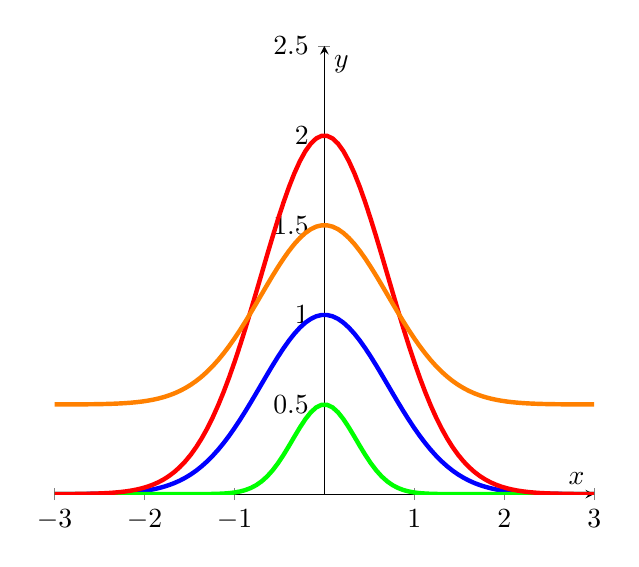
\begin{tikzpicture}[scale=1.0]
        \begin{axis}[
            axis x line=middle,
            axis y line=middle,
            ymin=0,ymax=2.5,ylabel=$y$,
            xmin=-3,xmax=3,xlabel=$x$
            ]

            \addplot[domain=-3:3, blue, ultra thick, samples=100] {e^(-x^2)};
            \addplot[domain=-3:3, green, ultra thick, samples=100] {0.5*e^(-(2*x)^2)};
            \addplot[domain=-3:3, red, ultra thick, samples=100] {2*(e^(-x^2))};
            \addplot[domain=-3:3, orange, ultra thick, samples=100] {e^(-x^2) + 0.5};
        \end{axis}
    \end{tikzpicture}
\caption{Amplitude transformations}
\label{fig:amplitude-scale-shifts}
\end{figure}

Given a signal $f(t)$, $f(at)$ will \emph{scale} the time domain by a factor of $\frac{1}{a}$, while $f(t - b)$ will \emph{shift} the time domain by $b$. Note that the opposite transformation is applied to the signal than is directly applied to the function inputs. Figure \ref{fig:time-scale-shifts} shows a signal $f(t)$ in blue, as well as:
\begin{itemize}
    \item $f(2t)$ in red,
    \item $f(\frac{t}{2})$ in green,
    \item and $f(t - 1)$ in orange.
\end{itemize}

It is important to note the different between scaling and then shifting the time of the signal, versus shifting and then scaling. Figure \ref{fig:time-scale-shifts-2} shows a signal $f(t)$ in blue, as well as:
\begin{itemize}
    \item $f(2(t-1))$ in red,
    \item and $f(2t-1)$ in green.
\end{itemize}

\begin{figure}[ht!]
    \centering
    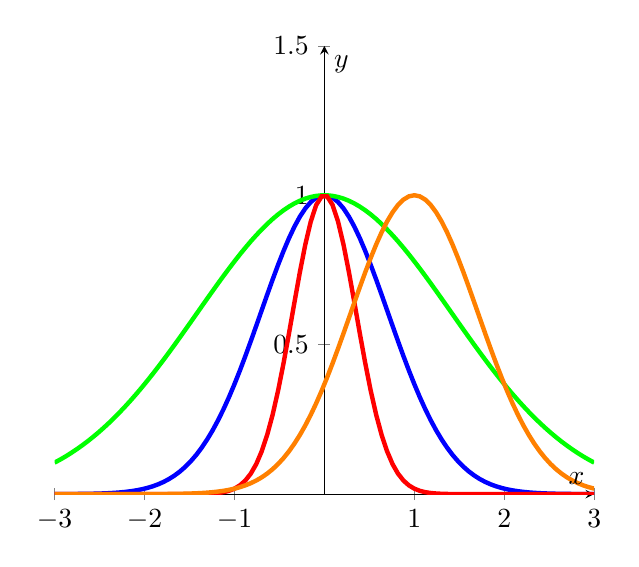
\begin{tikzpicture}[scale=1.0]
        \begin{axis}[
            axis x line=middle,
            axis y line=middle,
            ymin=0,ymax=1.5,ylabel=$y$,
            xmin=-3,xmax=3,xlabel=$x$
            ]

            \addplot[domain=-3:3, blue, ultra thick, samples=100] {e^(-x^2)};
            \addplot[domain=-3:3, green, ultra thick, samples=100] {e^(-(x/2)^2)};
            \addplot[domain=-3:3, red, ultra thick, samples=100] {(e^(-(2*x)^2))};
            \addplot[domain=-3:3, orange, ultra thick, samples=100] {e^(-(x-1)^2)};
        \end{axis}
    \end{tikzpicture}
\caption{Time transformations}
\label{fig:time-scale-shifts}
\end{figure}

\begin{figure}[ht!]
    \centering
    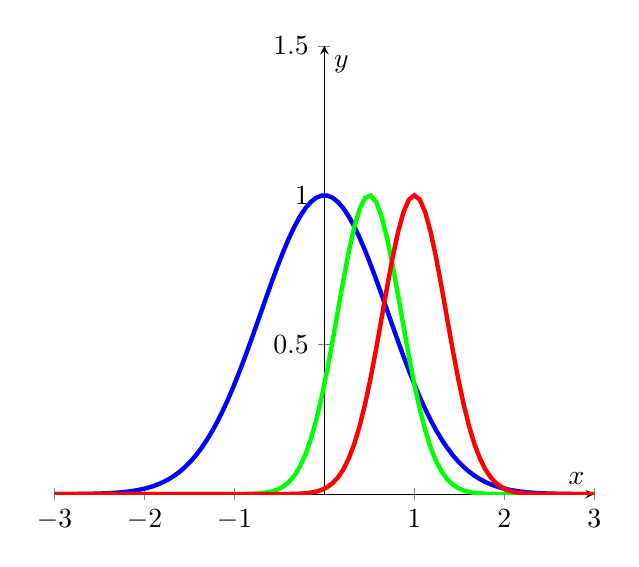
\begin{tikzpicture}[scale=1.0]
        \begin{axis}[
            axis x line=middle,
            axis y line=middle,
            ymin=0,ymax=1.5,ylabel=$y$,
            xmin=-3,xmax=3,xlabel=$x$
            ]

            \addplot[domain=-3:3, blue, ultra thick, samples=100] {e^(-x^2)};
            \addplot[domain=-3:3, green, ultra thick, samples=100] {e^(-(2*x-1)^2)};
            \addplot[domain=-3:3, red, ultra thick, samples=100] {e^(-(2*(x-1))^2};
        \end{axis}
    \end{tikzpicture}
\caption{Time transformations 2}
\label{fig:time-scale-shifts-2}
\end{figure}

\section{Common signals}

Two of the most common signals are the unit impulse signal, and the unit step signal. The unit impulse is also known as the (Dirac) delta function. In discrete time it is commonly denoted by $\delta[n]$, and is defined by
\[\delta[n] =
\begin{dcases}
    1, & n = 1 \\
    0, & n \neq 0
\end{dcases}.\] The unit step signal $u[n]$ is defined by
\[u[n] = \sum_{m=-\infty}^{n}\delta[m].\] Note that $\delta[n] = u[n] - u[n-1]$.

\begin{figure}[ht!]
    \centering
    \begin{tikzpicture}[scale=1.0]
        \begin{axis}[
            axis x line=middle,
            axis y line=middle,
            ymin=0,ymax=1.5,ylabel=$y$,
            xmin=-3,xmax=3,xlabel=$x$
            ]

            \addplot+[const plot, no marks, ultra thick] coordinates {(-3,0) (0,0) (0,1) (0,0) (3,0)};
        \end{axis}
    \end{tikzpicture}
\caption{Discrete unit impulse signal}
\label{fig:discrete-unit-impulse}
\end{figure}

\begin{figure}[ht!]
    \centering
    \begin{tikzpicture}[scale=1.0]
        \begin{axis}[
            axis x line=middle,
            axis y line=middle,
            ymin=0,ymax=1.5,ylabel=$y$,
            xmin=-3,xmax=3,xlabel=$x$
            ]

            \addplot+[const plot, no marks, ultra thick] coordinates {(-3,0) (0,0) (0,1) (3,1)};
        \end{axis}
    \end{tikzpicture}
\caption{Discrete unit step signal}
\label{fig:discrete-unit-step}
\end{figure}

The delta function can be used to sift out everything but one value of a discrete time signal.
\[x[n]\delta[n-n_0] = x[n_0]\delta[n-n_0]\]
\[\sum_{m=-\infty}^n x[m]\delta[m-n_0] = x[n_0]\]

In continuous time, we can define the unit step function similarly as \[u(t) =
\begin{dcases}
    1, & t > 0 \\
    0, & t < 0
\end{dcases}.\]
Note that $u(0)$ is undefined. Defining the continuous time impulse is a bit more challenging. We would like it to be $\delta(t)$ such that
\[u(t) = \int_{-t}^{t}\delta(\tau)d\tau.\] We can therefore define it has $\delta(t) = \lim_{\Delta\to 0}\delta_{\Delta}(t)$, where $\delta_{\Delta}(t)$ is a step impulse with width $\Delta$ and height $\frac{1}{\Delta}$ beginning at $t = 0$.

Note the similarities between the discrete and continuous time version of these signals -- the first difference and first derivative play the same roles, as do the sums and integrals.

\section{Energy and power}

\begin{defn}
    Let $x(t)$ be a continuous time signal. The \emph{energy} of the signal is
    \[E_{\infty} = \lim_{T\to\infty}\int_{-T}^{T}\abs{x(t)}^2dt.\]
\end{defn}

\begin{defn}
    Let $x(t)$ be a continuous time signal. The \emph{power} of the signal is
    \[P_{\infty} = \lim_{T \to \infty}\frac{1}{2T}\int_{-T}^T\abs{x(t)}^2dt.\]
\end{defn}

\begin{defn}
    Let $x[n]$ be a discrete time signal. The \emph{energy} of the signal is
    \[E_{\infty} = \lim_{N\to\infty}\sum_{n=-N}^{N}\abs{x[n]}^2.\]
\end{defn}

\begin{defn}
    Let $x[n]$ be a discrete time signal. The \emph{power} of the signal is
    \[P_{\infty} = \lim_{N \to \infty}\frac{1}{2N+1}\sum_{n=-N}^N\abs{x[n]}^2.\]
\end{defn}

Note that if a signal has finite energy, then the signal must approach zero sufficiently fast as time approaches $\pm\infty$, or equal zero outside some interval.

\begin{defn}
    An \emph{energy signal} is a signal with finite energy. Such signals must have zero power.
\end{defn}

\begin{exmp}
    $x(t) = e^{-\abs{t}}$ is an energy signal.
\end{exmp}

\begin{defn}
    A \emph{power signal} is a signal with finite, non-zero power. Such signals must have infinite energy.
\end{defn}

\begin{exmp}
    $x(t) = 1$ is a power signal, as is $x(t) = \sin(t)$.
\end{exmp}

Some signals are neither energy nor power signals, such as $x(t) = e^t$ or $x(t) = t$.

\begin{exmp}
    Let $x(t) = e^{-at}u(t)$ for some $a > 0$.
    \[E_{\infty} = \int_{-\infty}^{\infty}\abs{x(t)}^2dt = \int_{0}^{\infty}e^{-2at}dt = \frac{1}{-2a}(0 - 1) = \frac{1}{2a}.\] Since $a > 0$, $x(t)$ is therefore an energy signal and has zero power.
\end{exmp}

\begin{exmp}
    Let $x(t) = u(t)$. Then we have
    \[P_{\infty} = \lim_{T\to\infty}\frac{1}{2T}\int_{-T}^{T}\abs{x(t)}^2dt = \lim_{T\to\infty}\frac{1}{2T}\int_{0}^{T}dt = \frac{1}{2}.\] Therefore, $x(t)$ is a power signal and has infinite energy.
\end{exmp}

\section{Even and odd}

Recall that a function $f$ is even if $f(x) = f(-x)$ for all $x$ and odd if $f(x) = -f(-x)$. Obviously most functions are neither, but all functions can be decomposed into the sum of an even and odd part.

\begin{defn}
    Let $f(x)$ be a function, such as a signal. The \emph{even part} of $f$ is \[f_{\mathrm{ev}}(x) = \frac{f(x) + f(-x)}{2},\] and the \emph{odd part} of $f$ is \[f_{\mathrm{od}}(x) = \frac{f(x) - f(-x)}{2}.\]
\end{defn}

Note that the even part of a function must be even, since \[f_{\mathrm{ev}}(-x) = \frac{f(-x) + f(x)}{2} = \frac{f(x) + f(-x)}{2} = f_{\mathrm{ev}}(x),\] and the odd part must be odd: \[-f_{\mathrm{od}}(-x) = \frac{-f(-x)+f(x)}{2} = \frac{f(x) - f(-x)}{2} = f_{\mathrm{od}}(x).\]

\begin{exmp}
    $5x^2$ is even, while $x^3$ is odd, but $f(x) = x^3 + 5x^2$ is neither. \[f_{\mathrm{ev}}(x) = \frac{(x^3 + 5x^2) + ((-x)^3) + 5(-x)^2)}{2} = \frac{(x^3 - x^3) + (5x^2 + 5x^2)}{2} = 5x^2.\]
    \[f_{\mathrm{od}}(x) = \frac{(x^3 + 5x^2) - ((-x)^3) + 5(-x)^2)}{2} = \frac{(x^3 + x^3) + (5x^2 - 5x^2)}{2} = x^3.\]
\end{exmp}

\begin{prop}
    Let $f(x)$ be a function. Then $f(x) = f_{\mathrm{ev}}(x) + f_{\mathrm{od}}(x)$.
\end{prop}

\begin{proof}
    \begin{align*}
        f_{\mathrm{ev}}(x) + f_{\mathrm{od}}(x) &= \\
        \frac{f(x) + f(-x)}{2} + \frac{f(x) - f(-x)}{2} &= \\
        \frac{f(x) + f(-x) + f(x) - f(-x)}{2} &= \\
        \frac{2f(x)}{2} = f(x)
    \end{align*}
\end{proof}

\section{Period and frequency}

\begin{defn}
    A signal $x(t)$ is \emph{bounded} if there exists some $K$ such that $\abs{x(t)} < K$ for all $t$.
\end{defn}

\begin{defn}
    A signal $x(t)$ is \emph{periodic} if there exists some $T \in \R$ such that $x(t) = x(t + T)$ for all $T$. Note that if $f(t)$ is periodic with period $T$, it must also be periodic with period $kT$ where $k \in \Z^+$. The smallest such $T$ is called $T_0$, the \emph{fundamental period}.
\end{defn}

\begin{rmk}
    For discrete time signals, it is instead required that $T \in \Z^+$.
\end{rmk}

\begin{rmk}
    Constant signals are somewhat of an edge case with respect to periodicity. They are clearly periodic for any period $T > 0$, but have no fundamental period, and hence no fundamental frequency.
\end{rmk}

\begin{defn}
    Given that $x(t)$ is periodic with fundamental period $T_0$, the \emph{fundamental frequency} of $x(t)$ is $\omega_0 = \frac{2\pi}{T_0}$. Some sources instead call $f_0$ the fundamental frequency where $f_0 = \frac{1}{T_0}$.
\end{defn}

\begin{exmp}
    Let $x(t) = \sin(3t)$. If $x(t)$ is periodic with some period $T$, then it must be that $x(t) = x(t + T)$, so $\sin(3t) = \sin(3(t + T)) = \sin(3t + 3T)$. We know that $\sin$ is periodic with fundamental period $2\pi$, so $3T_0 = 2\pi$ and therefore $T_0 = \frac{2\pi}{3}$.
\end{exmp}

\begin{exmp}
    Let $x(t) = e^{\pi(1 + j)t}$. Then we have $x(t) = x(t + T)$ which implies \[e^{\pi(1 + j)t} = e^{\pi(1 + j)(t + T)} = e^{\pi(1 + j)t}e^{\pi(1 + j)T}.\] Since $e^x \neq 0$ for all $x$, it follows that $e^{\pi(1 + j)T} = 1$, and so it must be that $\pi(1 + j)T = 2k{\pi}$ for some $k \in \Z$ by Euler's formula. Therefore, $T = \frac{2k}{1 + j}$. However, $T \notin \R$, so $x(t)$ is not periodic.
\end{exmp}

\begin{rmk}
    If a \emph{non-zero} signal is both \emph{periodic} and \emph{bounded}, it must be a power signal.
\end{rmk}

\begin{rmk}
    Signals which are periodic in continuous time may not be in discrete time. For example, we saw that $x(t) = \sin(3t)$ is periodic, but $x[n] = \sin(3n)$ is not, as there is no $N \in \Z^+$ such that $N = \frac{2\pi}{3}$.
\end{rmk}

\section{Exponential signals}

\subsection{Continuous time}

\begin{defn}
    An \emph{exponential signal} is a signal of the form $x(t) = ce^{at}$, for some $c, a \in \C$ and $t \in \R$.
\end{defn}

When $c, a \in \R$, the exponential signal is similar to the standard exponential function. If $a > 0$, the signals grows exponentially, if $a < 0$ it decreases exponentially, and in any case it is scaled by $c$.

When $c \in \C$ and $a$ is strictly imaginary, the signal is called a \emph{phasor}. By Euler's formula, we have \[ce^{at} = \abs{c}e^{i\phi_0}e^{at} = \abs{c}e^{i(\omega_0t + \phi_0)} = \abs{c}\left(\cos(\omega_0t + \phi_0) + i\sin(\omega_0t + \phi_0)\right),\] where $i\omega_0 = a$ and $\phi_0 = \angle c$. A phasor can be interpreted as a vector-valued function, which always have magnitude $\abs{c}$, and has angular frequency $\omega_0$ (radians/time). At time $t = 0$, the angle is $\phi_0$, which may be called the \emph{phase} of the signal. Since the signal has angular frequency $\omega_0$, it has fundamental period $T_0 = \frac{2\pi}{\abs{w_0}}$.

\begin{thm}
    Let $x(t) = c_1e^{i\omega_1t} + c_2e^{i\omega_2t}$. This signal is periodic if and only if there exists some $\omega > 0$ and $k_1, k_2 \in \Z$ such that $\omega_1 = k_1\omega$ and $\omega_2 = k_2\omega$. If it is periodic, it has fundamental period $T_0 = \frac{2\pi}{\omega_0}$, where $\omega_0$ is the largest possible value for $\omega$.
\end{thm}

\begin{rmk}
    The required condition is equivalent to $\frac{\omega_1}{\omega_2} \in \Q$. Note that this theorem can be generalized to signals that are the sum of $n$ phasors.
\end{rmk}

\begin{exmp}
    Let $x(t) = 4e^{i2t} - 5e^{i3t}$. Since $2 = 2\cdot 1$ and $3 = 3 \cdot 1$, $x(t)$ is periodic with fundamental frequency $w_0 = 1$ and fundamental period $T_0 = \frac{2\pi}{\abs{1}} = 2\pi$.
\end{exmp}

\begin{exmp}
    Let $x(t) = 4e^{i2t} - 5e^{i\pi t}$. Since $\frac{2}{\pi} \not\in \Q$, $x(t)$ is not periodic.
\end{exmp}

\begin{defn}
    If a signal $x(t) = c_1e^{i\omega_1t} + c_2e^{i\omega_2t} + \cdots + c_ke^{i\omega_kt}$ is periodic, then we say the terms are \emph{harmonically related}.
\end{defn}

When $c, a \in \C$, and $a$ is not strictly imaginary, then the resulting exponential signal is a phasor given by $c$ and the imaginary part of $a$, all multiplied by $e^{\sigma_0}$, where $\sigma_0$ is the real part of $a$.

\subsection{Discrete time}

\begin{defn}
    An \emph{exponential signal} is a signal of the form $x[n] = ce^{an}$, for some $c, a \in \C$ and $n \in \N$.
\end{defn}

When $c, a \in \R$, the exponential signal is similar to the standard exponential function. If $a > 0$, the signals grows exponentially, if $a < 0$ it decreases exponentially, and in any case it is scaled by $c$.

When $c \in \R$ and $a = \sigma_0 + i(2k+1)\pi$ for some $\sigma_0 \in \R$ and $k \in \Z$, we have a type of exponential signal that doesn't have a continuous time version. Since $x[n] = ce^{an}$, we have $x[n] = c\left(-e^{\sigma_0}\right)^n$. This signal therefore is simply $ce^{n\sigma_0}$, but alternating between positive and negative on each sample.

When $c \in \C$ and $a$ is strictly imaginary, the signal is a discrete time \emph{phasor}. Unlike continuous time phasors, discrete time phasors are not always periodic. For $x[n] = e^{i\omega_0n}$ to be periodic in discrete time, we need $\frac{2\pi}{\abs{\omega_0}} \in \Q$, so that some integer multiple of this value is an integer period.

\begin{thm}
    Let $x[n] = c_1e^{i\omega_1n} + c_2e^{i\omega_2n}$, where the terms are periodic with fundamental periods $N_1, N_2 \in \N$. This signal is then periodic, and has fundamental period equal to the least common multiple of $N_1$ and $N_2$.
\end{thm}

\begin{rmk}
    Note that this theorem can be generalized to signals that are the sum of $n$ discrete time phasors.
\end{rmk}

\begin{rmk}
    For a continuous time phasors, increasing $\omega_0$ always results in a phasor with higher frequency. For a discrete time phasor however, add integer multiples of $2\pi$ to $\omega_0$ least the phasor unchanged.
\end{rmk}

\end{document}
